%! TEX root = 'main.tex'
\section{Design}
\label{sec:design}
In this section, we introduce the overall design and each major components in this toy CPU.

\subsection{Design Specification}
To make the design simple enough so that we can fully understand, 8-bit processor seems to be a good choice. Because a byte has 8 bits, a 4-bit processor can be cumbersome when reading/writing memory. It needs to read/write the memory twice for one byte, and the 4-bit register cannot store the entire byte. After deciding the processor is 8-bit, next, we want to make a 8-bit, fixed length instruction set. It's much easier to decode and to fetch instructions compares to variable length instruction set as in x86 architecture.

The following is our design specification, based on the 8-bit setting.

\begin{itemize}
	\item 8-bit instruction
	\item 8-bit general register
	\item 4-bit memory address
	\item Shared 4-bit address bus and 8-bit data bus (share 8 lines)
	\item Control signals (control bus)
\end{itemize}

The CPU has one 4-bit program counter (PC), one 8-bit instruction register (IR), two 8-bit general register, one arithmetic logic unit (ALU), one memory address register (MAR), one output register and 16-byte static memory (SRAM). These components are all connected to an 8-bit bus. It also has a control logic module that issues control signals to all the components. The overall view of the CPU's schematic is shown in~\autoref{fig:cpu}.  

\begin{figure}[th]
	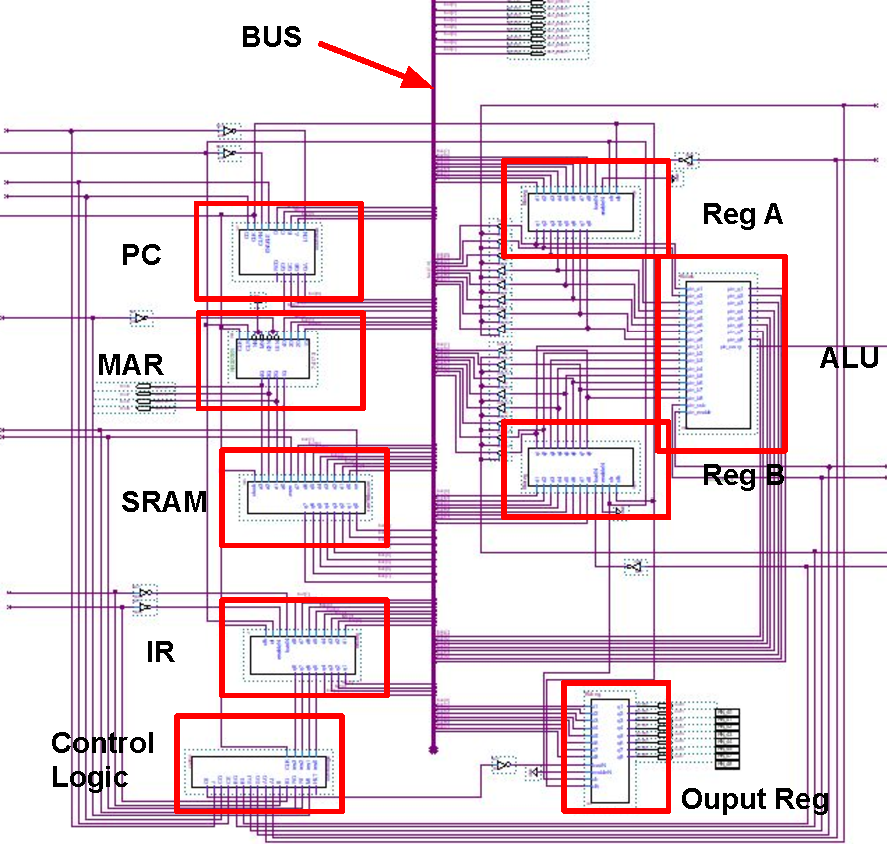
\includegraphics[width=0.47\textwidth]{figures/cpu}
	\centering
	\caption{The overall view of the CPU}
	\label{fig:cpu}
\end{figure}

The thick line in the middle is the bus which has 8 lines. It transfers both address and data. All the component connects to the bus, that is, all components can be connected to each other through the bus. And this is achieved through the control logic module. We will explain it in more detail in the following sections.


\subsection{Instruction Set}

Now we can create instruction set by ourselves. First we have to determine the format of the instruction. The upper 4-bit is opcode. All instructions have at most one operand, and this operand is a 4-bit memory address, as shown in~\autoref{fig:opcode}. There is no register operand, so some instructions have a default register. This design also leads us to only one memory addressing mode.

\begin{figure}[th]
	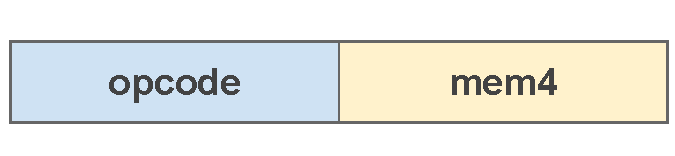
\includegraphics[width=0.47\textwidth]{figures/opcode}
	\centering
	\caption{8-bit instruction, 4-bit for opcode and 4-bit for memory operand.}
	\label{fig:opcode}
\end{figure}

Currently, we have only implemented 6 instructions, as shown below.

\begin{itemize}
	\item	NOP : No operation
	\item	LDA mem4 : Load memory into register A
	\item	ADD mem4 : Load memory then add it to register A
	\item	DISPLAY\_CFG : Send configuration data to 1602A LCD~\cite{1602a}
	\item	OUT : Send data to 1602A LCD
	\item	HLT : Halt
\end{itemize}

\subsection{Register}
The CPU has two general registers and one instruction register which are 8-bit. The MAR is 4-bit due to the memory space we have.

For 4-bit register, we use 74173 TTL logic module that provided by the FPGA software Quartus. 74713 is a 4-bit D-type register with 3-state outputs. For 8-bit register, we put two 74173 in parallel to form one 8-bit register, as shown in~\autoref{fig:8bitreg}.

\begin{figure}[th]
	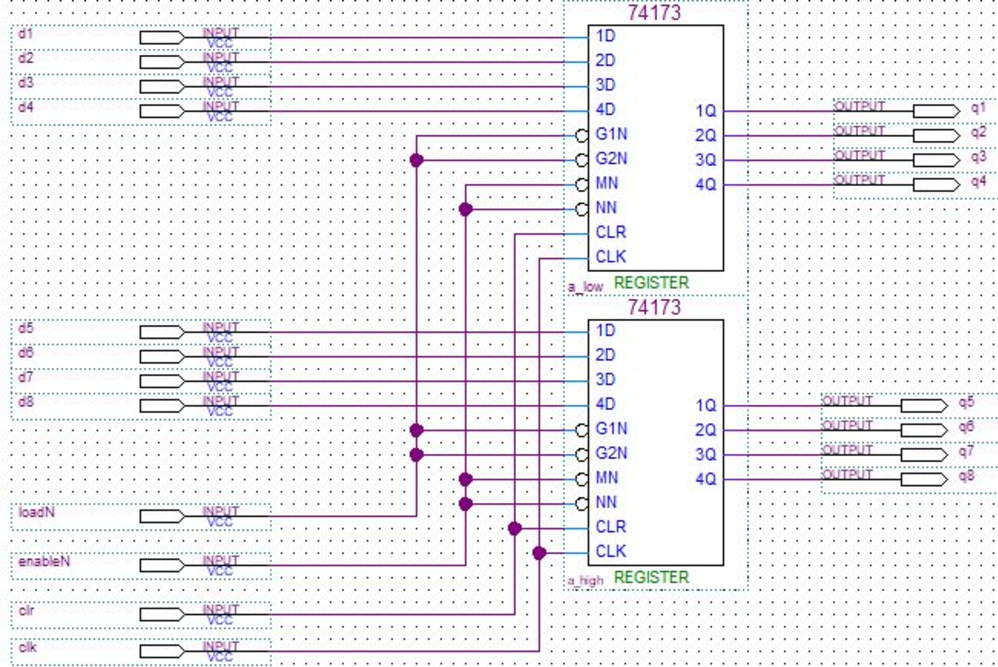
\includegraphics[width=0.47\textwidth]{figures/8bitreg}
	\centering
	\caption{8-bit register is composed of two 4-bit registers in parallel.}
	\label{fig:8bitreg}
\end{figure}


\subsection{MAR and Memory}

In this simple CPU, we do not use dynamic memory (DRAM) but static memory (SRAM). First, we are not sure whether FPGA can simulate capacitors and thus implement DRAM. Secondly, the CPU on modern computers runs much faster than memory, which requires a chipset to control it separately, or a CPU with a memory controller. We are not clear about these concepts yet, so we use SRAM to make memory and CPU work on the same frequency. This memory is quit similar to L1 instruction cache in modern computers, it only take one clock cycle to read/write. (Actually, because we use the memory module provided by Quartus, it takes 2 clock cycle to read/write. This is reflected in the control logic in our source code. But for simplicity, later in~\autoref{sec:casestudy}, we assume that the memory only takes one clock cycle to read/write data)


The memory address register either stores the memory address from which data will be fetched from the memory module, or the address to which data will be sent to store. Basically, MAR holds the memory location of data that needs to be accessed. Since the CPU only have 16 bytes memory space, the MAR only needs 4-bit. As shown in~\autoref{fig:marmem}, the MAR's input (d) connects to bus and it's output (q) connects to the memory module. There is only one signal for MAR. 
\begin{itemize}
	\item MI (MAR IN)
\end{itemize}
When it is signaled, the MAR loads 4-bit data from bus. There is no MAR OUT signal, which means MAR always output current value to the memory module.

\begin{figure}[th]
	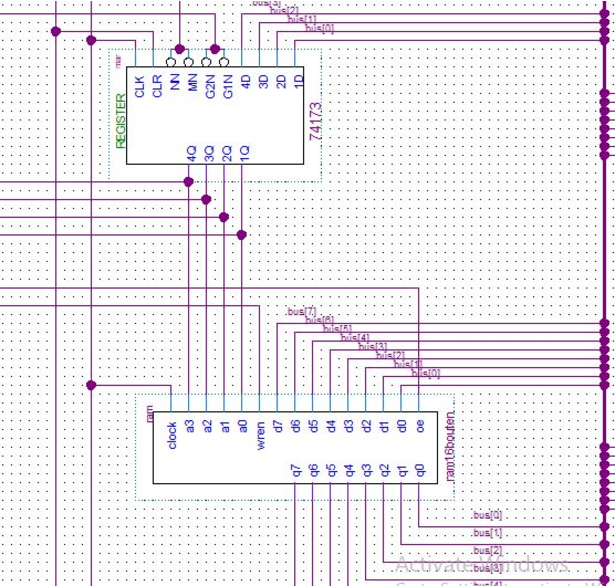
\includegraphics[width=0.47\textwidth]{figures/marmem}
	\centering
	\caption{MAR's input connects to bus and output connects to memory module.}
	\label{fig:marmem}
\end{figure}

The memory module's input (d) and output (q) are all connected with the bus. There are two control signals.

\begin{itemize}
	\item RI (RAM IN)
	\item RO (RAM OUT)
\end{itemize}

When RI is signaled, data will be sent to the memory. When RO is signaled, memory outputs data to the bus.


\subsection{IR}
IR is the register that holds the instruction being executed or decoded. Decoding the opcode in the instruction register includes determining the instruction, determining where its operands in memory, retrieving the operands from memory, allocating processor resources to execute the command, etc. In this case, as mentioned earlier, the low 4-bit is the only memory operand, so it will be output to the bus. The high 4-bit output of the IR is available to control logic, which generate the timing control signal that controls various processing components involved in executing the instruction. ~\autoref{fig:ir} shows that its input (d) connects to the bus, and its output (q) is divided into two parts, the low 4-bit part is sent to the bus, the high 4-bit part which is the opcode is sent to the control logic.

\begin{figure}[th]
	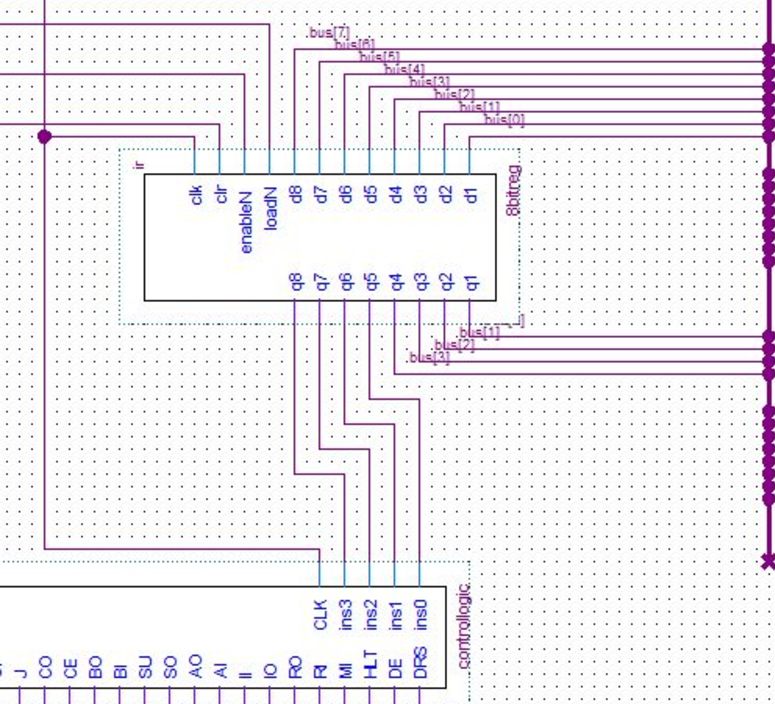
\includegraphics[width=0.47\textwidth]{figures/ir}
	\centering
	\caption{IR's input connects to bus and output to both bus and control logic.}
	\label{fig:ir}
\end{figure}

It has two control signals.

\begin{itemize}
	\item II (IR IN)
	\item IO (IR OUT)
\end{itemize}

II controls when the IR gets the instruction from the bus. When IO is signaled, IR outputs to both bus and control logic.


\subsection{General Registers}

We have two general registers A and B. As shown in~\autoref{fig:genreg}, they are both connected to ALU module. Although they are called general-purpose registers, register A is special, it's also an accumulator register. Because our instruction set design is too simple, no operand is used to indicate the register, so the default register for some instructions such as "ADD mem4" is register A.
 
\begin{figure}[th]
	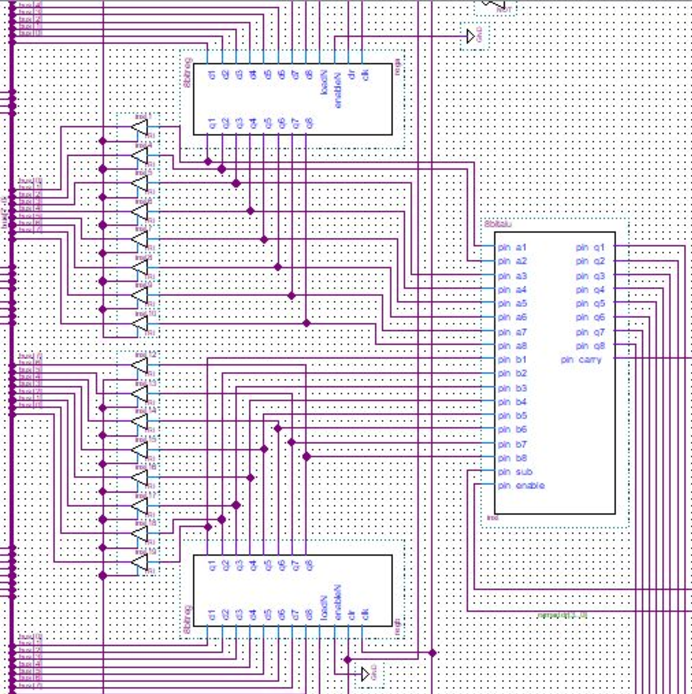
\includegraphics[width=0.47\textwidth]{figures/genreg}
	\centering
	\caption{Both general register A and B are connected to ALU and bus.}
	\label{fig:genreg}
\end{figure}

Each general register has two control signals, corresponding to the read and write of the register, as listed below.

\begin{itemize}
	\item AI (A IN)
	\item AO (A OUT)
	\item BI (B IN)
	\item BO (B OUT)
\end{itemize}



\subsection{PC}

The program counter (PC), commonly called the instruction pointer (IP) in Intel x86 microprocessors, and sometimes called the instruction address register (IAR) is a processor register that indicates where a CPU is in its program sequence.

Because our memory address space is only 16 bytes, the PC only needs 4 bits to cover the entire memory.

\begin{figure}[th]
	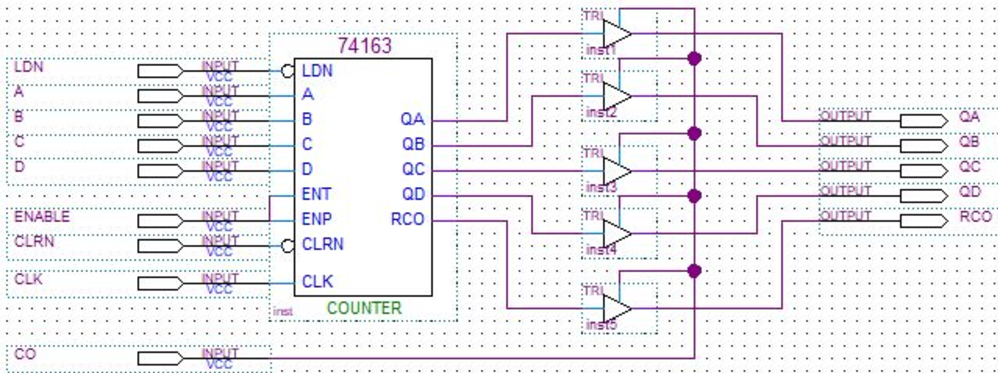
\includegraphics[width=0.47\textwidth]{figures/pc}
	\centering
	\caption{4-bit Program Counter}
	\label{fig:pc}
\end{figure}

We use 74163 4-bit counter as our program counter. Its 4-bit output will be sent to bus as a memory address to get one instruction from memory.

It also has two signals.

\begin{itemize}
	\item CE (COUNTER ENABLE)
	\item CO (COUNTER OUT)
\end{itemize}

When CO is signaled, the program counter output its content to the bus. Without CE signal, program counter will not increase on each clock cycle.


\subsection{Control Logic}

Their are 18 control signals in our design. The combination of signals can control the transmission of data between corresponding components. For example, issuing AO (A OUT) and BI (B IN) at the same clock cycle can make the data in register A transferred to register B. These signals can be regarded as atomic operations, and the function of control logic is to form a complete instruction through these operations.

Each instruction requires many clock cycles to complete, and several control signals need to be issued in each clock cycle. To do this, we use ROM to encode the instruction logics. Some instructions are more complicated and required more steps, and some instructions are relatively simple. So we set that each instruction needs to be completed in 6 steps. We use an 74163 4-bit counter to count the steps, as shown in~\autoref{fig:controllogic}.

\begin{figure}[th]
	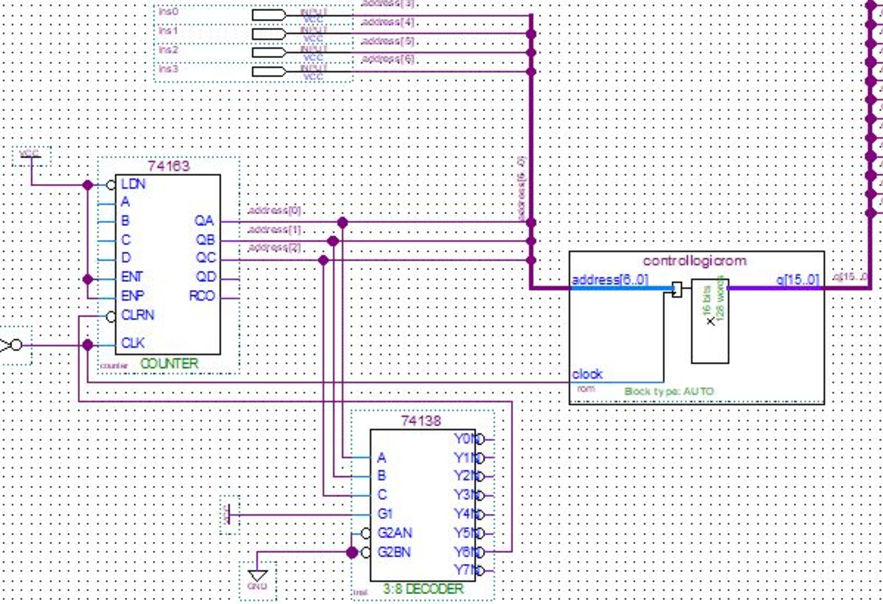
\includegraphics[width=0.47\textwidth]{figures/controllogic}
	\centering
	\caption{Control Logic Module}
	\label{fig:controllogic}
\end{figure}

The opcode of the instruction and each step number are encoded into an address. This address is used to index the data in the ROM. The data word width is 24 bits, which corresponds to 24 control signals. So far we have only used 18 of them.
